\chapter{Discussion}
Please tell more about conclusion and how to the next work of this study.
\section{Mhd Zulfikar Akram Nastuion / 1164081}
\subsection{Teori}
\begin{enumerate}

\item Jelaskan kenapa file teks harus di lakukan tokenizer. Dilengkapi dengan ilustrasi atau gambar !
\par
Sebelumnya kita harus tau terlebih dahulu apa itu Tokenizer. Tokenizer adalah sebuah proses pembagian terhadap kalimat yang berada dalam dokumen sehingga menjadi sebuah bagian - bagian kata atau bisa kita sebut denga token. Dalam dataset Youtube Tokenizer digunakan untuk melakukan vektorisasi data, sehingga dapat kita simpulkan bahwa data yang telah kita buat dokumen pada chapter 6 yaitu data spam dan bukan spam akan dilakukan vektorisasi dengan menggunakan Tokenizer ini. Ilustrasi sederhana mengenai Tokenizer ini misalkan saya memiliki sebuah kalimat Nama Saya Adalah Yusniar jika gunakan fungsi Tokenizer ini akan dipecah menjadi kata per kata, perhatikan figure \ref{1}.

	\begin{figure}[!htbp!]
		\centerline{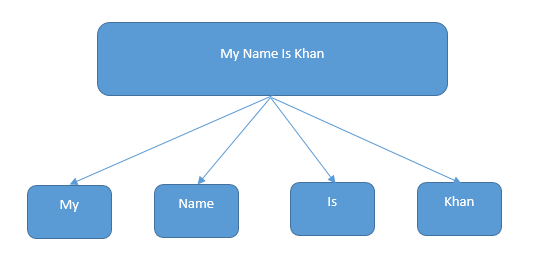
\includegraphics[width=0.5\textwidth]{figures/zulfikar/7/Teori/1164081_1.png}}
		\caption{Contoh Tokenizer.}
		\label{1}
	\end{figure}
\item Jelaskan konsep dasar K Fold Cross Validation pada dataset komentar Youtube pada source code dibawah. Dilengkapi dengan ilustrasi atau gambar !
	\lstinputlisting [firstline=3, lastline=4]{src/zulfikar/Teori/zulfikar7.py}
\par
Pada variabel kfold berisikan StratifieldKFold yang dimana akan diisikan sebuah sempel dan dibagi menjadi 5 dengan nsplits pada setiap class. Lalu akan dibuat variabel baru yang dinamakan dengan 2splits dan disikan class dari dataset Youtube. Pada data yang telah dilakukan split akan diperoleh hasil presentase akhir. Ilustrasi yang saya berikan misalkan ada sebuah data lalu data tersebut akan dibagi menjadi data testing dan training lalu dilakukan fungsi Cross Validation untuk memperoleh hasil presentase akhir. Perhatikan figure \ref{2}.

	\begin{figure}[!htbp!]
		\centerline{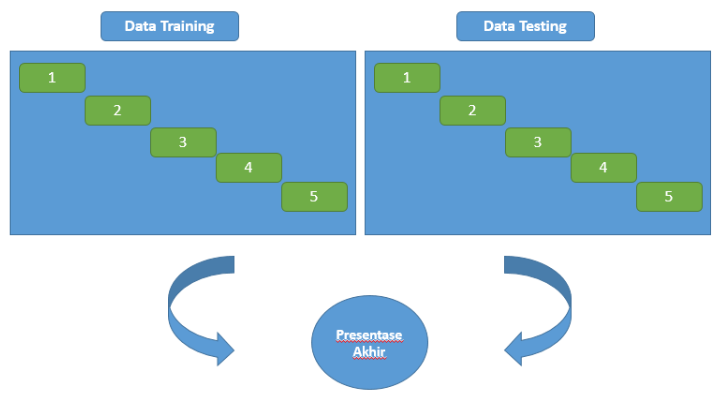
\includegraphics[width=0.5\textwidth]{figures/zulfikar/7/Teori/1164081_2.png}}
		\caption{Konsep Dasar K Fold Validation.}
		\label{2}
	\end{figure}
\item Jelaskan apa maksudnya kode program for train, test in splits. Dilengkapi dengan ilustrasi atau gambar !
\par
Dimana fungsi tersebut digunakan untuk melakukan pengujian terhadap data yang sudah di split atau belum dalam dataset dan tidak akan terjadi penumpukan, maksudnya pada setiap class tidak akan menampilkan id yang sama. Kali ini saya akan memberikan ilustrasi sederhana, misalkan ada seseorang yang ingin menyumbangkan buku cerita kepada perpustakan, lalu pihak perpustakaan akan menerimanya, dikarenakan yang di sumbangkan adalah buku cerita dan bermacam - macam maka tidak akan ada buku yang sama hal ini sama saja bisa dibilang tidak adanya id yang sama. Untuk ilustrasi nya perhatikan figure \ref{3}.

	\begin{figure}[!htbp!]
		\centerline{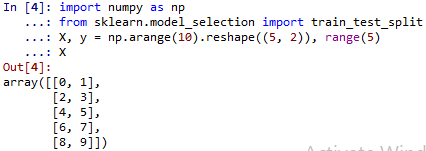
\includegraphics[width=0.5\textwidth]{figures/zulfikar/7/Teori/1164081_3.png}}
		\caption{Train And Test In Split.}
		\label{3}
	\end{figure}
\item Jelaskan apa yang dimaksud kode program dibawah. Dilengkapi dengan ilustrasi atau gambar !
\lstinputlisting[firstline=21, lastline=22]{src/zulfikar/Teori/zulfikar7.py}
Dimana source code tersebut akan mengambil data dari kolom Content yaitu kolom tersebut merupakan bagian dari train\_idx dan test\_idx. Ilustrasi yang saya berikan yaitu apabila kita telah mengubah suatu data menjadi data training atau data testing maka kita dapat menampilkan data tersebut dengan isi kolom yang kita mau.
\item Jelaskan apa maksud dari fungsi tokenizer = Tokenizer(num\_words=2000) dan tokenizer.fit\_on\_texts(train\_content), dilengkapi ilustrasi atau gambar !
\par
Variabel tokenizer tersebut akan melakukan proses vektorisasi kata sebanyak 2000 kata dengan menggunakan fungsi Tokenizer. Pada source code tokenizer.fit\_on\_texts(train\_content) akan melakukan fit dengan menggunakan fungsi tokenizer akan tetapi hanya pada data training saja pada kolom content. Untuk ilustrasi dapat dilihat pada figure \ref{4}

	\begin{figure}[!htbp!]
		\centerline{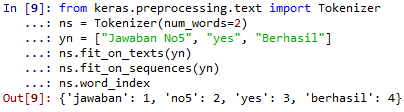
\includegraphics[width=0.5\textwidth]{figures/zulfikar/7/Teori/1164081_4.png}}
		\caption{Fungsi Tokenizer.}
		\label{4}
	\end{figure}
\item Jelaskan apa yang dimaksud dari fungsi source code dibawah !
\lstinputlisting[firstline=42, lastline=43]{src/zulfikar/Teori/zulfikar7.py}
\par
Pada source code baris pertama akan melakukan vektorisasi dari data training yang dimana data tersebut berbentuk string atau teks dan diubah kedalam bentuk matrix menggunakan model tdf. Untuk source code baris kedua akan melakukan vektorisasi data testing yang akan diubah kedalam bentuk matrix dengan mode tdf. Dimana kita ilustrasi source code nya adalah seperti yang ditampilkan pada figure \ref{5}.

	\begin{figure}[!htbp!]
		\centerline{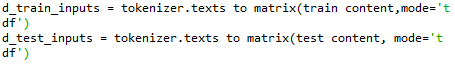
\includegraphics[width=0.5\textwidth]{figures/zulfikar/7/Teori/1164081_5.png}}
		\caption{Vektorisasi TDF Data Training Dan Testing.}
		\label{5}
	\end{figure}
\item Jelaskan apa yang dimaksud dari fungsi d\_train\_inputs = d\_train\_inputs/np.amax(np.absolute(d\_train)) dan  d\_test\_inputs = d\_test\_inputs/np.amax(np.absolute(d\_test)), dilengkapi dengan ilustrasi atau gambar !
\par
Pada source code tersebut akan melakukan pembagian data matrix yang sudah kita buat pada data trainig dan testing dan akan mengembalikan nilai maksimum array menggunakan class amax. Untuk ilustrasi dapat dilihat pada figure \ref{6}.

	\begin{figure}[!htbp!]
		\centerline{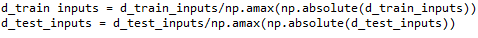
\includegraphics[width=0.5\textwidth]{figures/zulfikar/7/Teori/1164081_6.png}}
		\caption{Pembagian Data Matrix.}
		\label{6}
	\end{figure}
\item Jelaskan apa yang dimaksud fungsi d\_train\_outputs = np\_utils.to\_categorical(d[CLASS].iloc[train\_idx] dan  d\_test\_outputs = np\_utils.to\_categorical(d[CLASS].iloc[test\_idx] dalam kode program dilengkapi dengan ilustrasi atau gamabar !
\par
Source code tersebut digunakan untuk melakuakan fungsi yang dinamakan One-hot encoding yang nantinya data tersebut dapat digunakan dalam proses Neural Network. Data yang diambil terdiri dari CLASS yaitu Spam dan No Spam dari data training dan data testing. Untuk ilustrasi dapat dilihat pada figure \ref{7}.

	\begin{figure}[!htbp!]
		\centerline{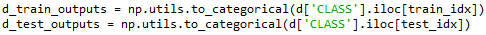
\includegraphics[width=0.5\textwidth]{figures/zulfikar/7/Teori/1164081_7.png}}
		\caption{One-hot Encoding.}
		\label{7}
	\end{figure}
\item Jelaskan apa yang dimaksud dengan dari fungsi source code dibawah,
\lstinputlisting[firstline=8, lastline=13]{src/zulfikar/Teori/zulfikar7.py}
\par
Source Code tersebut akan melakukan sequential yang diamana akan melakukan perbandingan pada setiap elemen secara satu persatu dan berurut. Terdapat 512 Neurons dengan jumlah input shape sebesar 2000 yang dimana sudah dilakukan normalisasi. Mpdel tersebut akan dilakukan aktivasi menggunakan model relu lalu dilakukan dropout atau pemotongan sebesar 50\%. Pada neurons selanjutnya terdapat 2  yang kemudian akan dilakukan aktivasi menggunakan fungsi softmax.
\item Jelaskan apa yang dimaksud dari fungsi pada source code dibawah dengan parameter tersebut !
\lstinputlisting[firstline=17, lastline=17]{src/zulfikar/Teori/zulfikar7.py}
\par
Source code tersebut akan melakukan proses compile dengan menggunakan fungsi optimizer dan memunculkan data loss dan akurasi matrix.

\item Jelaskan apa itu Deep Learning !
\par
Deep Learning merupakan sebuah cabang dari Mechine Learning dimana konesep yang deep learning ini hampir serupa dengan Mechine Learning hanya saja deep learning dilakukan dengan metode yang lebih cerdas, contohnya dalam menditeksi wajah itu termasuk deep learning.

\item Jelaskan apa itu Deep Neural Network dan apa bedanya dengan Deep Learning !
\par
Deep Neural Network merupakan sebuah algoritma berbasis Neural Netowork yang digunakan dalam pengambilan sebuah keputusan. Perbedaan DNN dengan DL antara lain DNN merupakan algoritma yang digunakan terhadap DL sedangkan DL yang akan menggunakan algoritma tersebut.
\item Jelaskan dengan ilustrasi gambar langkah per langkah bagaimana perhitungan algoritma konvolusi dengan ukuran stide (NPM mod 3 + 1) x (NPM mod 3 + 1) yang terdapat max pooling !

	\begin{itemize}
		\item Pertama tentukan nilai (x,y)
		\item Nilai tersebut dibuat kedalam bentuk matrix
		\item Jika sudah berbentuk matrix lakukan perkalian antar baris dan deret
		\item Berhubung dikarenakan matriksnya berordo 1 maka hasilnya menjadi matriks berordo 1 juga.
	\end{itemize}

	\subitem Untuk ilustrasi dapat dilihat pada figure \ref{8}

	\begin{figure}[!htbp!]
		\centerline{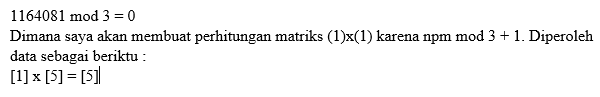
\includegraphics[width=0.5\textwidth]{figures/zulfikar/7/Teori/1164081_8.png}}
		\caption{Algoritma Konvolusi Dengan Matrix (1x1).}
		\label{8}
	\end{figure}	



\end{enumerate}